\section{Experiment}
\label{Experiment}
The experiment is performed to determine the function and performance of the whole system. The experiment program is simulated in a suitable system. This experiment is conducted to determine the reliability of the system and to determine whether it is in accordance with the planning or not. The experiment will be done that is in accordance with the step steps in Figure 1 and Figure 2.

\subsection{Hardware Used}
The modules have been compiled with all the required sequences and have been implemented with the required components. The overall design result of the tool and system can be seen in the following figure:
\begin{figure}[ht]
\begin{center}
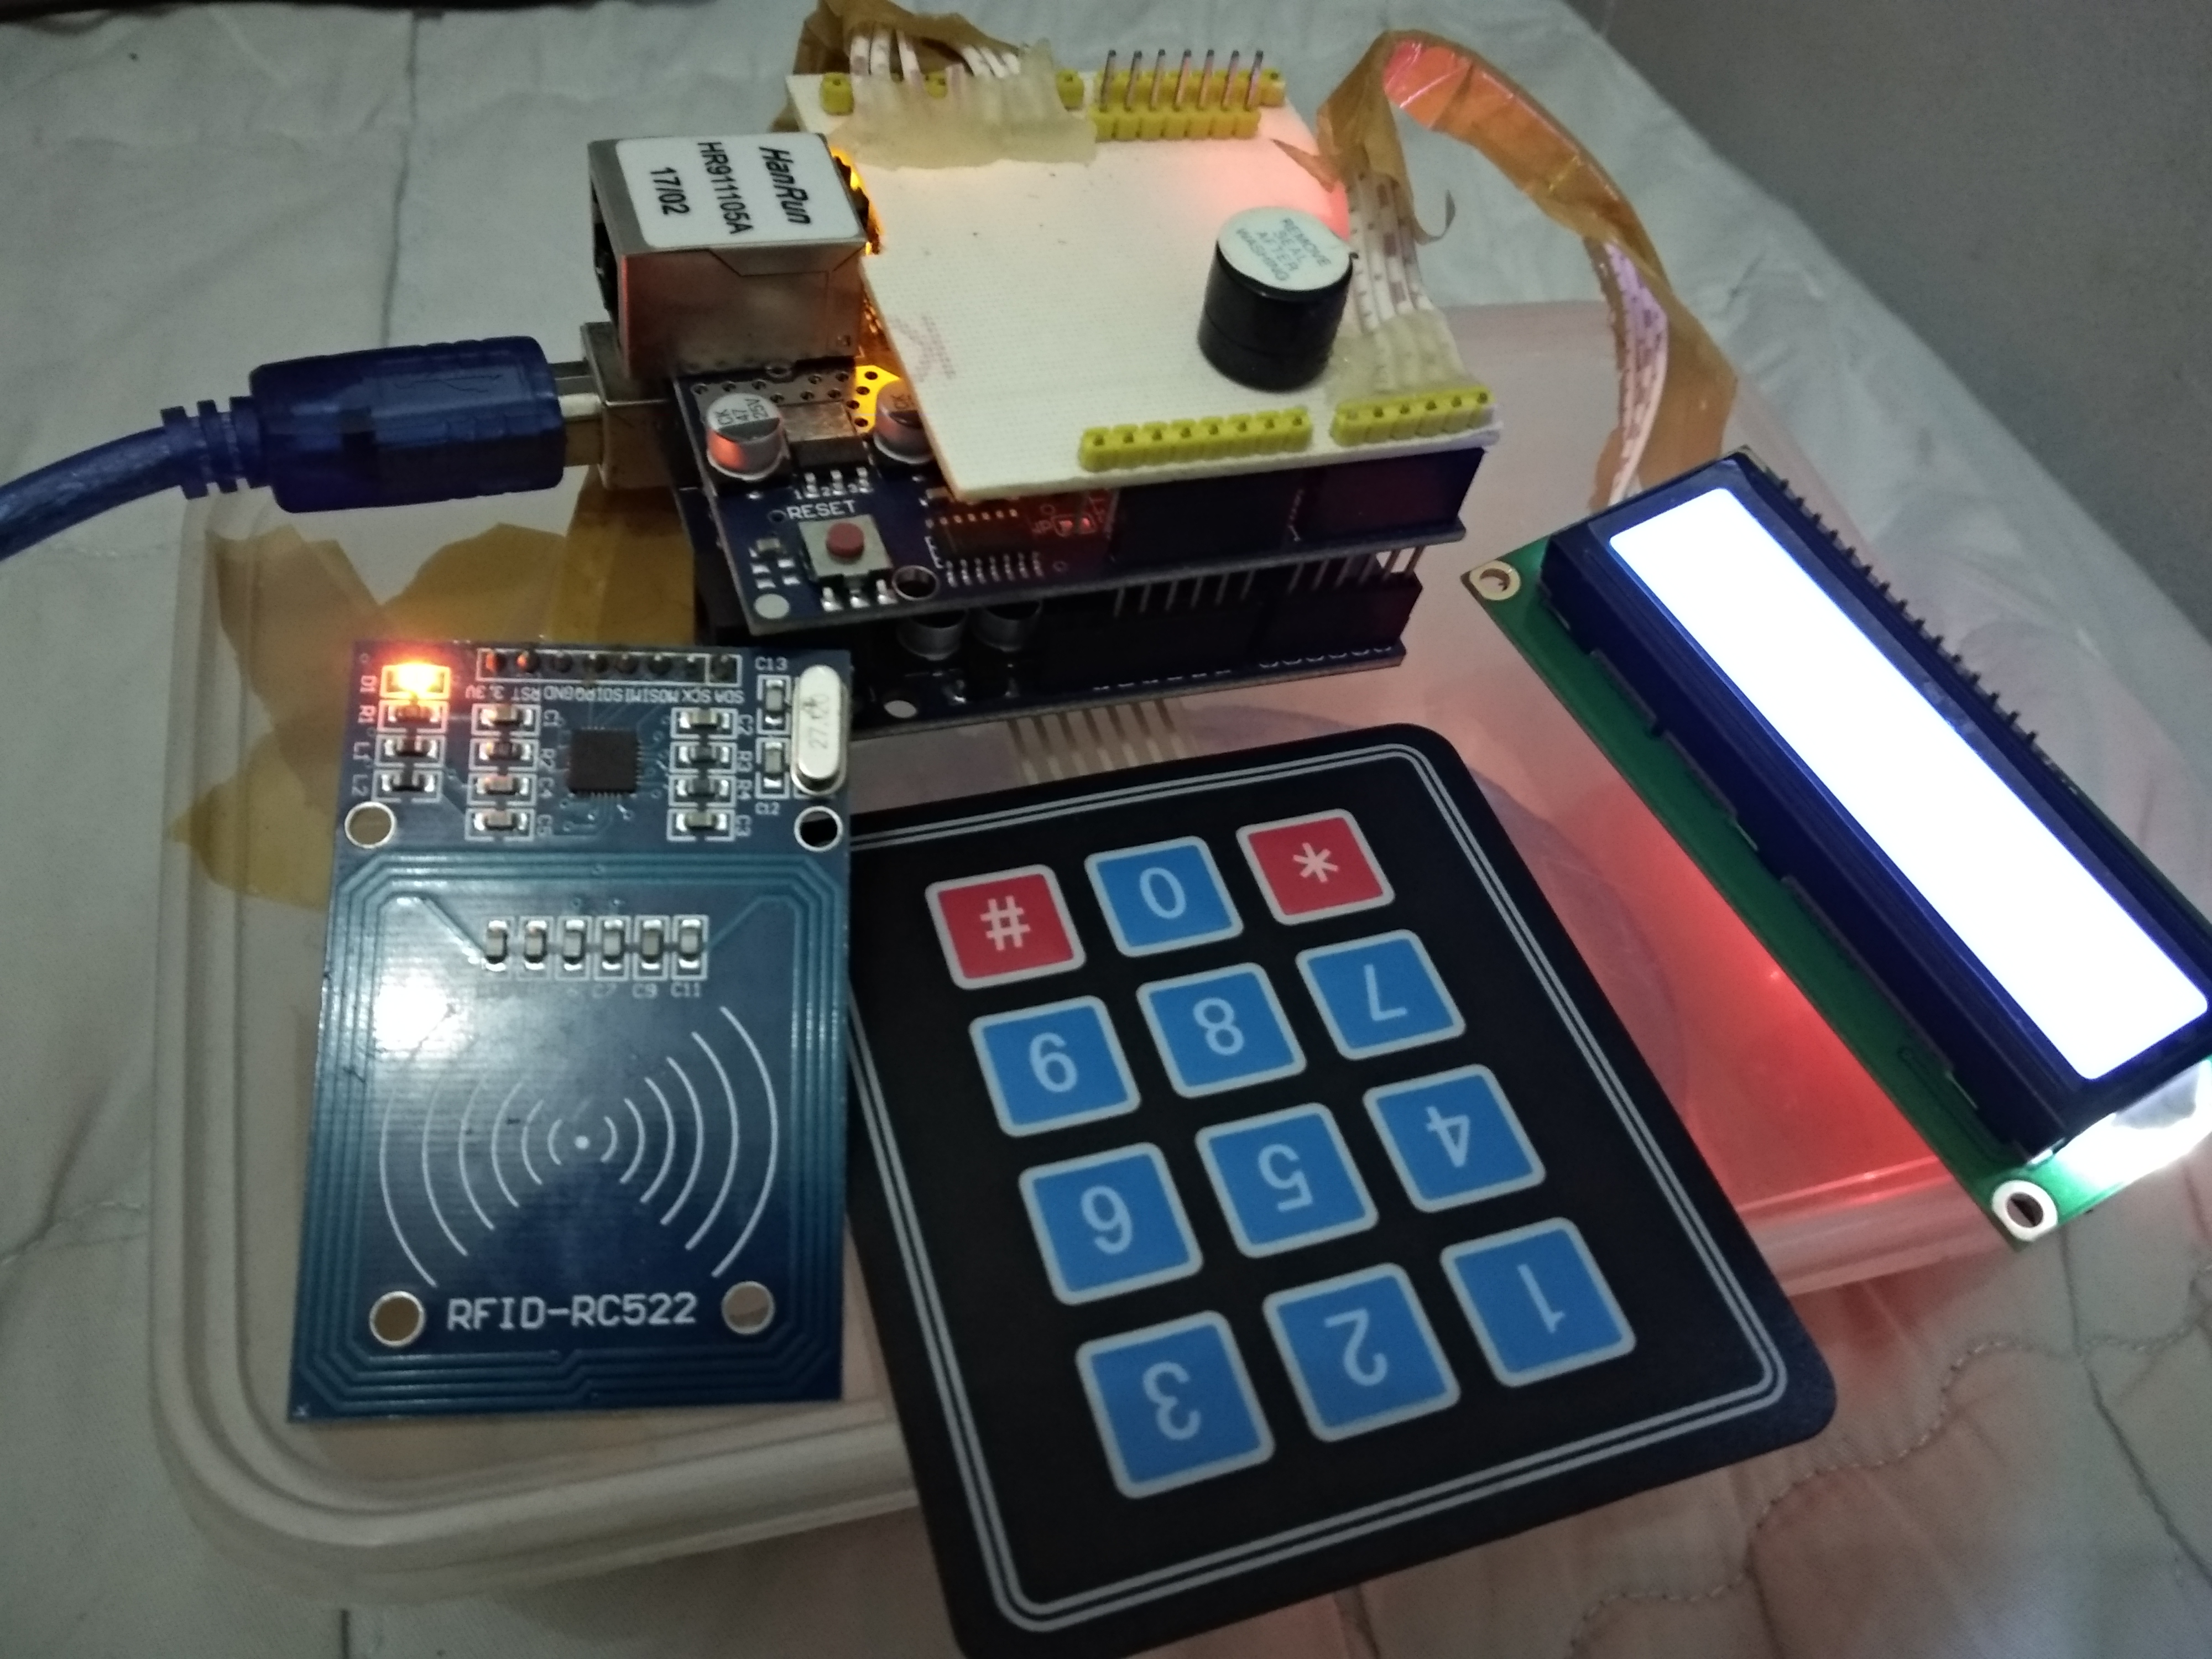
\includegraphics[width=8cm]{figures/Tools.jpg}
\end{center}
\caption{RFID Tools.
\label{eq:30}}
\end{figure} 

\subsection{Implementation Methods}
The application of the Multi-Factor Authentication method with the implementation of the OTP code is used to secure and verify the user. With this method user authentication will be performed.
The process of applying the method on this hardware is when the user tapping in the morning or early entry to work then the code will be sent to the user account based on the card ID, then when the clock home has arrived the user will do tapping and input the code on the keypad that has been provided.
After entering the OTP code 'hash' button on the keypad is pressed to transmit data and check the code in the database.

\begin{left}
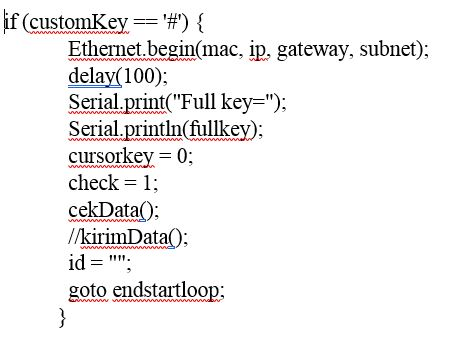
\includegraphics[width=6cm]{figures/COde1.JPG}
\end{left}

If wrong inserts the OTP key 'star' key on the keypad is pressed to delete the wrong number

\begin{left}
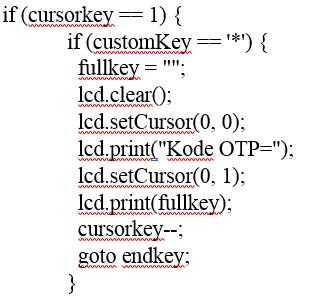
\includegraphics[width=4.5cm]{figures/COde2.JPG}
\end{left}


\subsection{Working of The System}
The concatenation in Figure 3 will be tested to perform user authentication process that is by way of initial entry, user will tapping rfid card to rfid reader. If the card has been registered with the OTP code will be sent to the user's account and the clock data entry will be stored on the database. And If the curfew, the user will be tapping an RFID card again and enter the code OTP had previously been sent to the account. Users will enter OTP code with a keypad that has been provided, if the code OTP appropriate then clock out successfully saved to the database, if it fails you will be notified if the code is entered incorrectly OTP.

If the card is not registered then the OTP code can not be sent and on the LCD will show the notification that the card used is not listed.

\begin{left}
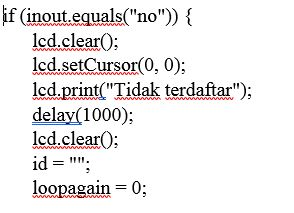
\includegraphics[width=5cm]{figures/COde3.JPG}
\end{left}

Furthermore, if the card is already registered but not feeding the notification that the OTP code is incorrect.

\begin{left}
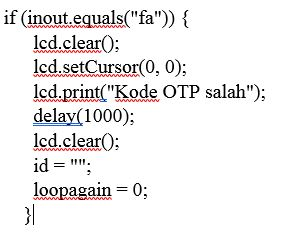
\includegraphics[width=4.5cm]{figures/COde4.JPG}
\end{left}

Therefore the system and Hardware will be interconnected with each other. Namely connected using ethernet and access to the system using the IP address is: 192.168.1.102.

\begin{left}
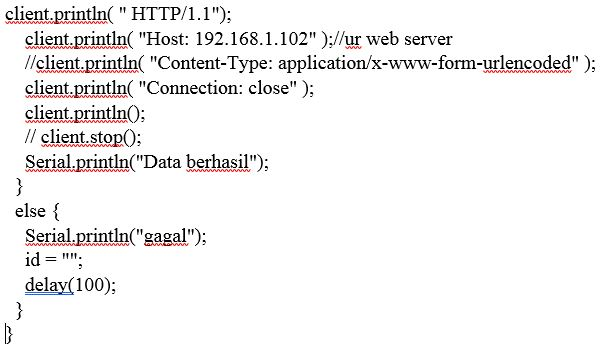
\includegraphics[width=8cm]{figures/COde5.JPG}
\end{left}